\clearpage
\section{Supplementary material}
\label{sec:3_supplement}
\renewcommand{\thefigure}{3.S\arabic{figure}}
\setcounter{figure}{0}


% Figure 3.S1 (misalignment)
% -------------------------
\begin{figure}[!tbh]
    \centering
    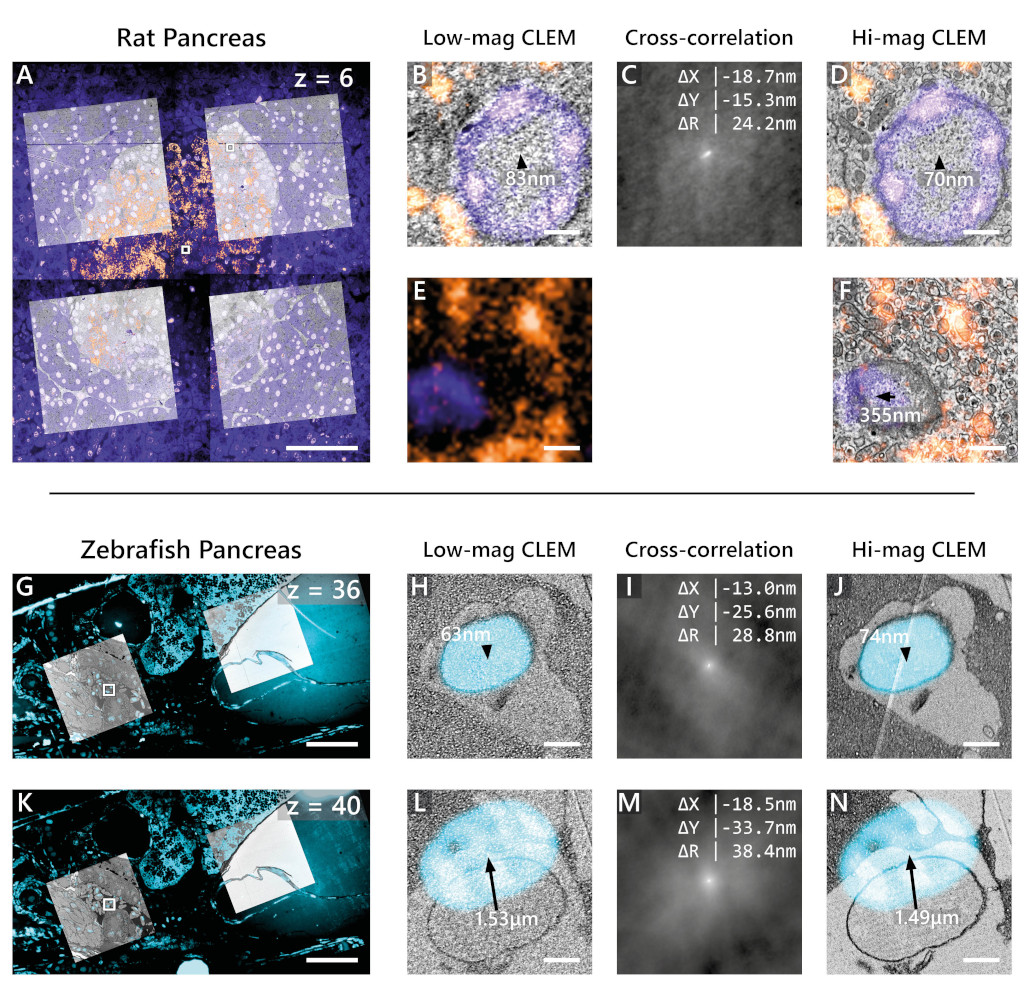
\includegraphics[width=\linewidth]{chapter-3/figures_JPEG_LQ/fig3-S1_misalignment.jpg}
    \caption{Reduced overlay accuracy due to extrapolation and errors in the CL registration procedure. Overlay (in)accuracy is a combination of the errors in the cross-modal and cross-spatial registration procedures.
    (A) Partial low-magnification CLEM tileset of rat pancreas from which features inside (B\,--\,D) and outside (E\,--\,F) a low-magnification EM tile were selected to assess the overlay accuracy (denoted by white squares).
    (B) Cross-modal registration error for a cell nucleus in low-magnification CLEM, measured by calculating the centroid of the nucleus in both modalities and computing the relative displacement.
    (C) Cross-spatial registration error as measured by the phase correlation between the low and high-magnification EM.
    (D) Sub-\SI{100}{\nano\meter} overlay accuracy for the cell nucleus in high-magnification CLEM.
    (E\,--\,F) Same as in (B) and (D) for a cell nucleus acquired outside of a low-magnification EM tile. Overlay accuracy is reduced to several hundred nanometers due to the imprecision incurred by extrapolating the cross-modal registration.
    (Continued on next page\ldots)}
    \label{fig:3.S1_misalignment}
\end{figure}
\addtocounter{figure}{-1}
\begin{figure}
    \caption{%
    (G) Partial low-magnification CLEM tileset of zebrafish pancreas from a section in which the CL registration procedure achieved the expected precision. (H\,--\,J) Same as in (B\,--\,D) but for a nucleus in the zebrafish pancreas. (K\,--\,N) Same as in (G\,--\,J) but for the section with the lowest apparent overlay accuracy (\SI{1.5}{\micro\meter}). The inaccuracy is dominated by an error in the cross-modal registration as the phase correlation (M) shows a sub-\SI{50}{\nano\meter} translation. Possible causes for the error include poor CL spot localization due to noise in the CL signal.
    Scale bars: (A) \SI{50}{\micro\meter}; (B, D, E, F) \SI{0.5}{\micro\meter}; (G, K) \SI{50}{\micro\meter}; (H, J, L, N) \SI{1}{\micro\meter}.}
\end{figure}

\quad
